\documentclass[]{article}
\usepackage{lmodern}
\usepackage{amssymb,amsmath}
\usepackage{ifxetex,ifluatex}
\usepackage{fixltx2e} % provides \textsubscript
\ifnum 0\ifxetex 1\fi\ifluatex 1\fi=0 % if pdftex
  \usepackage[T1]{fontenc}
  \usepackage[utf8]{inputenc}
\else % if luatex or xelatex
  \ifxetex
    \usepackage{mathspec}
  \else
    \usepackage{fontspec}
  \fi
  \defaultfontfeatures{Ligatures=TeX,Scale=MatchLowercase}
\fi
% use upquote if available, for straight quotes in verbatim environments
\IfFileExists{upquote.sty}{\usepackage{upquote}}{}
% use microtype if available
\IfFileExists{microtype.sty}{%
\usepackage{microtype}
\UseMicrotypeSet[protrusion]{basicmath} % disable protrusion for tt fonts
}{}
\usepackage[margin=1in]{geometry}
\usepackage{hyperref}
\PassOptionsToPackage{usenames,dvipsnames}{color} % color is loaded by hyperref
\hypersetup{unicode=true,
            pdftitle={空间广义线性混合效应模型及其在流行病预测中的应用},
            pdfauthor={黄湘云},
            pdfkeywords={R语言;混合模型;网络},
            colorlinks=true,
            linkcolor=Maroon,
            citecolor=Blue,
            urlcolor=Blue,
            breaklinks=true}
\urlstyle{same}  % don't use monospace font for urls
\usepackage{natbib}
\bibliographystyle{plainnat}
\usepackage{color}
\usepackage{fancyvrb}
\newcommand{\VerbBar}{|}
\newcommand{\VERB}{\Verb[commandchars=\\\{\}]}
\DefineVerbatimEnvironment{Highlighting}{Verbatim}{commandchars=\\\{\}}
% Add ',fontsize=\small' for more characters per line
\usepackage{framed}
\definecolor{shadecolor}{RGB}{248,248,248}
\newenvironment{Shaded}{\begin{snugshade}}{\end{snugshade}}
\newcommand{\KeywordTok}[1]{\textcolor[rgb]{0.13,0.29,0.53}{\textbf{#1}}}
\newcommand{\DataTypeTok}[1]{\textcolor[rgb]{0.13,0.29,0.53}{#1}}
\newcommand{\DecValTok}[1]{\textcolor[rgb]{0.00,0.00,0.81}{#1}}
\newcommand{\BaseNTok}[1]{\textcolor[rgb]{0.00,0.00,0.81}{#1}}
\newcommand{\FloatTok}[1]{\textcolor[rgb]{0.00,0.00,0.81}{#1}}
\newcommand{\ConstantTok}[1]{\textcolor[rgb]{0.00,0.00,0.00}{#1}}
\newcommand{\CharTok}[1]{\textcolor[rgb]{0.31,0.60,0.02}{#1}}
\newcommand{\SpecialCharTok}[1]{\textcolor[rgb]{0.00,0.00,0.00}{#1}}
\newcommand{\StringTok}[1]{\textcolor[rgb]{0.31,0.60,0.02}{#1}}
\newcommand{\VerbatimStringTok}[1]{\textcolor[rgb]{0.31,0.60,0.02}{#1}}
\newcommand{\SpecialStringTok}[1]{\textcolor[rgb]{0.31,0.60,0.02}{#1}}
\newcommand{\ImportTok}[1]{#1}
\newcommand{\CommentTok}[1]{\textcolor[rgb]{0.56,0.35,0.01}{\textit{#1}}}
\newcommand{\DocumentationTok}[1]{\textcolor[rgb]{0.56,0.35,0.01}{\textbf{\textit{#1}}}}
\newcommand{\AnnotationTok}[1]{\textcolor[rgb]{0.56,0.35,0.01}{\textbf{\textit{#1}}}}
\newcommand{\CommentVarTok}[1]{\textcolor[rgb]{0.56,0.35,0.01}{\textbf{\textit{#1}}}}
\newcommand{\OtherTok}[1]{\textcolor[rgb]{0.56,0.35,0.01}{#1}}
\newcommand{\FunctionTok}[1]{\textcolor[rgb]{0.00,0.00,0.00}{#1}}
\newcommand{\VariableTok}[1]{\textcolor[rgb]{0.00,0.00,0.00}{#1}}
\newcommand{\ControlFlowTok}[1]{\textcolor[rgb]{0.13,0.29,0.53}{\textbf{#1}}}
\newcommand{\OperatorTok}[1]{\textcolor[rgb]{0.81,0.36,0.00}{\textbf{#1}}}
\newcommand{\BuiltInTok}[1]{#1}
\newcommand{\ExtensionTok}[1]{#1}
\newcommand{\PreprocessorTok}[1]{\textcolor[rgb]{0.56,0.35,0.01}{\textit{#1}}}
\newcommand{\AttributeTok}[1]{\textcolor[rgb]{0.77,0.63,0.00}{#1}}
\newcommand{\RegionMarkerTok}[1]{#1}
\newcommand{\InformationTok}[1]{\textcolor[rgb]{0.56,0.35,0.01}{\textbf{\textit{#1}}}}
\newcommand{\WarningTok}[1]{\textcolor[rgb]{0.56,0.35,0.01}{\textbf{\textit{#1}}}}
\newcommand{\AlertTok}[1]{\textcolor[rgb]{0.94,0.16,0.16}{#1}}
\newcommand{\ErrorTok}[1]{\textcolor[rgb]{0.64,0.00,0.00}{\textbf{#1}}}
\newcommand{\NormalTok}[1]{#1}
\usepackage{graphicx,grffile}
\makeatletter
\def\maxwidth{\ifdim\Gin@nat@width>\linewidth\linewidth\else\Gin@nat@width\fi}
\def\maxheight{\ifdim\Gin@nat@height>\textheight\textheight\else\Gin@nat@height\fi}
\makeatother
% Scale images if necessary, so that they will not overflow the page
% margins by default, and it is still possible to overwrite the defaults
% using explicit options in \includegraphics[width, height, ...]{}
\setkeys{Gin}{width=\maxwidth,height=\maxheight,keepaspectratio}
\IfFileExists{parskip.sty}{%
\usepackage{parskip}
}{% else
\setlength{\parindent}{0pt}
\setlength{\parskip}{6pt plus 2pt minus 1pt}
}
\setlength{\emergencystretch}{3em}  % prevent overfull lines
\providecommand{\tightlist}{%
  \setlength{\itemsep}{0pt}\setlength{\parskip}{0pt}}
\setcounter{secnumdepth}{5}
% Redefines (sub)paragraphs to behave more like sections
\ifx\paragraph\undefined\else
\let\oldparagraph\paragraph
\renewcommand{\paragraph}[1]{\oldparagraph{#1}\mbox{}}
\fi
\ifx\subparagraph\undefined\else
\let\oldsubparagraph\subparagraph
\renewcommand{\subparagraph}[1]{\oldsubparagraph{#1}\mbox{}}
\fi

%%% Use protect on footnotes to avoid problems with footnotes in titles
\let\rmarkdownfootnote\footnote%
\def\footnote{\protect\rmarkdownfootnote}

%%% Change title format to be more compact
\usepackage{titling}

% Create subtitle command for use in maketitle
\newcommand{\subtitle}[1]{
  \posttitle{
    \begin{center}\large#1\end{center}
    }
}

\setlength{\droptitle}{-2em}
  \title{空间广义线性混合效应模型及其在流行病预测中的应用}
  \pretitle{\vspace{\droptitle}\centering\huge}
  \posttitle{\par}
\subtitle{Spatial Generalized Linear Mixed Models and its Applications to
Prevlence Mapping}
  \author{黄湘云}
  \preauthor{\centering\large\emph}
  \postauthor{\par}
  \date{}
  \predate{}\postdate{}

\usepackage{\usepackage{ctex}}

\begin{document}
\maketitle
\begin{abstract}
空间广义线性混合效应模型的应用背景介绍\\
空间广义线性混合效应模型及其应用\\
空间广义线性混合效应模型及其应用
\end{abstract}

{
\hypersetup{linkcolor=black}
\setcounter{tocdepth}{4}
\tableofcontents
}
\section{论文综述}

线性模型 到 广义线性模型 线性混合效应模型 到 广义线性混合效应模型 再到
空间广义线性混合效应模型

求解混合效应模型的各种方法

从 kriging 克里金插值 到 高斯过程

简单介绍提出本文的大纲思路

简单回顾广义线性模型和混合效应模型

定位统计计算

广义线性模型的应用广泛 广义线性模型的算法实现进展综述

介绍空间数据统计包含地统计、离散空间变差、空间点过程

引出广义线性模型在geostatistical data analysis 的应用及算法实现

在 S 语言中空间数据分析和建模 Modern Applied Statistics with S
\citep{MASS2002}

检验环境和基因效应在空间相关性中的存在性 \citep{spaMM2014}
流行现象的时空分析\citep{surveillance2017}

近年来涉及空间数据分析和建模的书籍也越来越多,

用于空间数据分析的分层模型 Hierarchical Modeling and Analysis for
Spatial Data \citep{Banerjee2015}

基于R-INLA软件的空间和时空贝叶斯模型 Spatial and Spatio-temporal
Bayesian Models with R-INLA \citep{Blangiardo2015}

特别地,基于地统计数据的有 \citep{Schl2016Using}

R 语言空间数据可视化方面呈现越来越流行的趋势,从早些年的 lattice
\citep{lattice2008} 到如今的 ggplot2\citep{ggplot22016},操作空间数据的
sp 对象也发展为 sf 对象,同时整合了不少第三方软件和服务 如基于 Google
Earth 的空间可视化 \citep{plotKML2015} ,基于Google Maps的交互空间可视化
\citep{plotGoogleMaps2012}

一元和多元时空模型spBayes包 \citep{spBayes2015}

\section{模型介绍}

\subsection{线性模型}

线性模型的一般形式为

\begin{equation}
Y = X'\beta + \epsilon, \mathsf{E}(\epsilon) = 0, \mathsf{Cov}(\epsilon) = \sigma^2 I \label{eq:LM}
\end{equation}

其中,\(Y = (y_1,y_2,\cdots,y_n)'\) 是 \(n\)
维列向量,代表对响应变量\(Y\)的\(n\)次重复观测;\(\beta = (\beta_0,\beta_1,\cdots,\beta_{p-1})'\)
是 \(p\) 维列向量,代表模型自变量 \(X\) 的系数,\(\beta_0\)是截距项;
\(X' = (1_{(1\times n)}',X_{(1)}',X_{(2)}',\cdots,X_{(n)}')\),\(1_{(1\times n)}'\)
是全1的\(n\)维列向量,而\(X_{(i)}' = (x_{1i},x_{2i},\cdots,x_{ni})'\)
代表对第\(i\)个自变量的\(n\)次观测;
\(\epsilon = (\epsilon_1,\epsilon_2,\cdots,\epsilon_n)'\)是\(n\)
维列向量,代表模型的随机误差,\(\mathsf{E}(\epsilon_i \epsilon_j) = 0, i \ne j\)。
求解线性模型 \eqref{eq:LM} 的 R 函数是
\texttt{lm},近年来,高维乃至超高维稀疏线性模型成为热门的研究方向,相关的R包也越来越多,比较著名的有\texttt{glmnet}\citep{glmnet2011JSS}
和 \texttt{SIS}\citep{SIS2016JSS}。

\subsection{广义线性模型}

广义线性模型的一般形式

\begin{equation}
Y \sim \mathtext{指数族} \quad
\eta = X'\beta \quad
\mathsf{E}(Y) = g^{-1}(\eta)  \label{eq:GLM}
\end{equation}

简写之为

\begin{equation*}
g(\mu) = X'\beta
\end{equation*}

其中\(\mu \equiv \mathrm{E}(Y)\), \(g\) 代表联系函数,特别地,当
\(Y \sim N(\mu,\sigma^2)\) 时,\(g(x) = x\) ;当
\(Y \sim \mathsf{Binomial}(n,p)\) 时,\(g(x)=\ln(\frac{x}{1-x})\);当
\(Y \sim \mathsf{Possion}(\lambda)\)
时,\(g(x) = \ln(x)\);此处不一一列举。\citep{McCullagh1989}
模型\eqref{eq:GLM}最早由 Nelder 和 Wedderburn
\citep{Nelder1972}提出,它弥补了模型\eqref{eq:LM}
的两个重要缺点:一是因变量只能取连续值的情况,二是期望与自变量只能用线性关系联系
\citep{Chen2011}。求解广义线性模型 \eqref{eq:GLM} 的 R 函数是
\texttt{glm},参数估计的办法一般是拟似然法。

\subsection{混合效应模型}

广义线性混合模型的一般形式

\begin{equation}
g(\mu) = X'\beta + Z'b  \label{eq:GLMM}
\end{equation}

其中 \(Z'\) 是\(q\)维随机效应的 \(n \times q\) 的向量值矩阵。
混合效应模型包含线性混合效应模型、广义线性混合效应模型、非线性混合效应模型等,之所以称之为混合效应,是因为模型既包含固定效应(fixed-effects)又随机效应(random
effects)。如前所述的线性和广义线性模型中的自变量就是固定效应,而随机效应是那些不能直接观察到的潜变量。求解模型\eqref{eq:GLMM}的R包有
\texttt{nlme} \citep{R-nlme},\texttt{mgcv} \citep{mgcv2017}
和\texttt{lme4}\citep{lme4JSS},参数估计的方法一般有限制极大似然法。

\subsection{空间广义线性混合效应模型}

本文重点关注空间广义线性混合效应模型(Spatial Generalized linear
mixed-effects
models,简写为SGLMM)\citep{Zhang2002On, Varin2005Pairwise, Bonat2016Practical},它既是对模型\eqref{eq:LM}、\eqref{eq:GLM}和\eqref{eq:GLMM}的延伸也是对空间数据分析的应用,属于空间统计下的地统计(geostatistics)分支,因此在有些参考文献\citep{Diggle2002, Christensen2004, Diggle2007}中也称为广义线性地统计模型(Generalized
linear geostatistical models),SGLMM
具有广泛的应用,如分析核污染浓度的空间分布\citep{Diggle1998},预测热带流行病的分布\citep{Diggle2016}

\section{算法描述}

\subsection{贝叶斯方法}

coda: Convergence Diagnosis and output analysis for MCMC
用于对MCMC的收敛性诊断和输出分析 \citep{coda2006} geoR:
用于空间数据分析和预测的贝叶斯方法 \citep{geoR2001} geoRglm:
空间广义线性混合效应模型 \citep{geoRglm2002} brms \citep{brms2017JSS}

\begin{Shaded}
\begin{Highlighting}[]
\KeywordTok{library}\NormalTok{(coda)}
\end{Highlighting}
\end{Shaded}

MCMCvis--- Tools to Visualize, Manipulate, and Summarize MCMC Output

Performs key functions for MCMC analysis using minimal code -
visualizes, manipulates, and summarizes MCMC output. Functions support
simple and straightforward subsetting of model parameters within the
calls, and produce presentable and `publication-ready' output. MCMC
output may be derived from Bayesian model output fit with JAGS, Stan, or
other MCMC samplers.

mgcv and JAGS

Stan 是一种概率编程语言\citep{Stan2017JSS},可以替代 BUGS (
\textbf{B}ayesian inference \textbf{U}sing \textbf{G}ibbs
\textbf{S}ampling ) \citep{BUGS} 作为 MCMC
的高效实现,可用于贝叶斯框架下,标准地统计模型的参数估计,Stan
提供多种语言的接口实现,方便起见,本文采用它提供的 R 语言接口 -- rstan
包 \citep{Stan2015, Stan2017JSS}。此外,还有\citep{rethinking2015}  

lme4 \citep{lme4JSS}

gstat \citep{gstat2016}

glmmBUGS RStan 实现MCMC

\subsection{最大似然方法}

最大似然 \citep{PrevMap2017} 将 MCML 和 MCMC
方法应用于空间广义线性混合效应模型的参数估计和预测,

\subsection{拉普拉斯近似}

方法 \citep{Rue2017arXiv}

\section{数值模拟}

\texttt{RandomFields}是模拟多元随机场的 R 包 \citep{RandomFields2015},
\texttt{geoR} 包\citep{R-geoR2016}的 \texttt{grf}
函数只适合模拟少量数据点

分泊松、二项两种情况、上述3种方法,在空间广义线性混合效应模型下的模拟情况(使用标准的地统计模型,无时间项和混合分布)

标准地统计流行抽样模型(Standard Geostatistical Prevalence Sampling
Model)

\begin{equation}
\log[p(x_i)/\{1-p(x_i)\}] = d(x_i)'\beta + S(x_i) + Z_i \label{eq:SGPSM}
\end{equation}

其中 \(\mathsf{S} = \{S(x):x \in \mathbb{R}^2\}\)

\begin{Shaded}
\begin{Highlighting}[]
\NormalTok{####################################}
\CommentTok{# 模拟空间广义线性混合效应模型}
\NormalTok{####################################}
\KeywordTok{library}\NormalTok{(mvtnorm)}
\KeywordTok{library}\NormalTok{(geoR) }
\NormalTok{## --------------------------------------------------------------}
\NormalTok{##  Analysis of Geostatistical Data}
\NormalTok{##  For an Introduction to geoR go to http://www.leg.ufpr.br/geoR}
\NormalTok{##  geoR version 1.7-5.2 (built on 2016-05-02) is now loaded}
\NormalTok{## --------------------------------------------------------------}
\KeywordTok{library}\NormalTok{(RandomFields)}
\NormalTok{## Loading required package: sp}
\NormalTok{## Loading required package: RandomFieldsUtils}
\NormalTok{## }
\NormalTok{## Attaching package: 'RandomFieldsUtils'}
\NormalTok{## The following object is masked from 'package:geoR':}
\NormalTok{## }
\NormalTok{##     matern}
\NormalTok{## }
\NormalTok{## Attaching package: 'RandomFields'}
\NormalTok{## The following object is masked from 'package:RandomFieldsUtils':}
\NormalTok{## }
\NormalTok{##     RFoptions}
\NormalTok{## The following objects are masked from 'package:base':}
\NormalTok{## }
\NormalTok{##     abs, acosh, asin, asinh, atan, atan2, atanh, cos, cosh, exp,}
\NormalTok{##     expm1, floor, gamma, lgamma, log, log1p, log2, logb, max, min,}
\NormalTok{##     round, sin, sinh, sqrt, tan, tanh, trunc}
\KeywordTok{set.seed}\NormalTok{(}\DecValTok{2018}\NormalTok{)}
\NormalTok{N <-}\StringTok{ }\DecValTok{400} \CommentTok{# 样本量}
\CommentTok{# N <- 10000 }
\CommentTok{# 模拟二元正态分布}
\NormalTok{sigma <-}\StringTok{ }\KeywordTok{matrix}\NormalTok{(}\KeywordTok{c}\NormalTok{(}\DecValTok{2}\NormalTok{, .}\DecValTok{2}\NormalTok{, .}\DecValTok{2}\NormalTok{, }\DecValTok{3}\NormalTok{), }\DataTypeTok{byrow =} \OtherTok{TRUE}\NormalTok{, }\DataTypeTok{ncol =} \DecValTok{2}\NormalTok{) }\CommentTok{# 协方差矩阵  }
\NormalTok{data.x <-}\StringTok{ }\KeywordTok{cbind}\NormalTok{(}\KeywordTok{rep}\NormalTok{(}\DecValTok{1}\NormalTok{, N), }\KeywordTok{rmvnorm}\NormalTok{(}\DataTypeTok{n =}\NormalTok{ N, }\DataTypeTok{mean =} \KeywordTok{c}\NormalTok{(}\DecValTok{1}\NormalTok{, }\DecValTok{2}\NormalTok{), }\DataTypeTok{sigma =}\NormalTok{ sigma))}
\NormalTok{beta <-}\StringTok{ }\KeywordTok{c}\NormalTok{(}\FloatTok{1.2}\NormalTok{, }\DecValTok{1}\NormalTok{, }\FloatTok{0.2}\NormalTok{) }\CommentTok{# 模型系数 其中 beta_0 = 1.2 是截距  }
\CommentTok{# 添加空间随机效应 sigma^2 = 1 phi = 25 tau^2 =1 kappa = 1}
\NormalTok{S <-}\StringTok{ }\KeywordTok{grf}\NormalTok{(N, }\DataTypeTok{grid =} \StringTok{"irreg"}\NormalTok{, }\DataTypeTok{nx =}\NormalTok{ N, }\DataTypeTok{ny =}\NormalTok{ N,}
        \DataTypeTok{xlims =} \KeywordTok{c}\NormalTok{(}\DecValTok{0}\NormalTok{,}\DecValTok{100}\NormalTok{), }\DataTypeTok{ylims =} \KeywordTok{c}\NormalTok{(}\DecValTok{0}\NormalTok{,}\DecValTok{100}\NormalTok{), }\DataTypeTok{nsim =} \DecValTok{1}\NormalTok{, }\DataTypeTok{mean=}\DecValTok{0}\NormalTok{,}
        \DataTypeTok{cov.mode =} \StringTok{"powered.exponential"}\NormalTok{,}
        \DataTypeTok{cov.par =} \KeywordTok{c}\NormalTok{(}\DecValTok{1}\NormalTok{,}\DecValTok{25}\NormalTok{), }\DataTypeTok{nugget =} \DecValTok{1}\NormalTok{, }\DataTypeTok{kappa =} \DecValTok{1}\NormalTok{)}
\NormalTok{## grf: simulation(s) on randomly chosen locations with  400  points}
\NormalTok{## grf: process with  1  covariance structure(s)}
\NormalTok{## grf: nugget effect is: tausq= 1 }
\NormalTok{## grf: covariance model 1 is: powered.exponential(sigmasq=1, phi=25, kappa = 1)}
\NormalTok{## grf: decomposition algorithm used is:  cholesky }
\NormalTok{## grf: End of simulation procedure. Number of realizations: 1}
\CommentTok{# 响应变量服从二项分布        }
\NormalTok{mu <-}\StringTok{ }\KeywordTok{exp}\NormalTok{(S}\OperatorTok{$}\NormalTok{data }\OperatorTok{+}\StringTok{ }\NormalTok{data.x }\OperatorTok\StringTok{ }\NormalTok{beta)}\OperatorTok{/}\NormalTok{(}\DecValTok{1} \OperatorTok{+}\StringTok{ }\KeywordTok{exp}\NormalTok{(S}\OperatorTok{$}\NormalTok{data }\OperatorTok{+}\StringTok{ }\NormalTok{data.x }\OperatorTok\StringTok{ }\NormalTok{beta))}
\NormalTok{binom.data.y <-}\StringTok{ }\KeywordTok{rbinom}\NormalTok{(N, }\DataTypeTok{size =} \DecValTok{10}\NormalTok{, }\DataTypeTok{prob =}\NormalTok{ mu) }\OperatorTok{/}\StringTok{ }\DecValTok{10}

\KeywordTok{ggplot}\NormalTok{(}\DataTypeTok{data =} \KeywordTok{as.data.frame}\NormalTok{(S}\OperatorTok{$}\NormalTok{coords), }\KeywordTok{aes}\NormalTok{(}\DataTypeTok{x =}\NormalTok{ x, }\DataTypeTok{y =}\NormalTok{ y, }\DataTypeTok{colour =}\NormalTok{ binom.data.y)) }\OperatorTok{+}\StringTok{ }
\StringTok{  }\KeywordTok{geom_point}\NormalTok{(}\DataTypeTok{pch =} \DecValTok{16}\NormalTok{, }\DataTypeTok{size =} \DecValTok{3}\NormalTok{, }\DataTypeTok{alpha =}\NormalTok{ .}\DecValTok{8}\NormalTok{) }\OperatorTok{+}\StringTok{  }
\StringTok{  }\KeywordTok{scale_colour_distiller}\NormalTok{(}\DataTypeTok{palette =} \StringTok{"Spectral"}\NormalTok{) }\OperatorTok{+}
\StringTok{  }\KeywordTok{labs}\NormalTok{(}\DataTypeTok{colour =} \StringTok{"观察概率"}\NormalTok{,}\DataTypeTok{x =} \StringTok{"横坐标"}\NormalTok{,}\DataTypeTok{y =} \StringTok{"纵坐标"}\NormalTok{)}
\end{Highlighting}
\end{Shaded}

\begin{figure}

{\centering 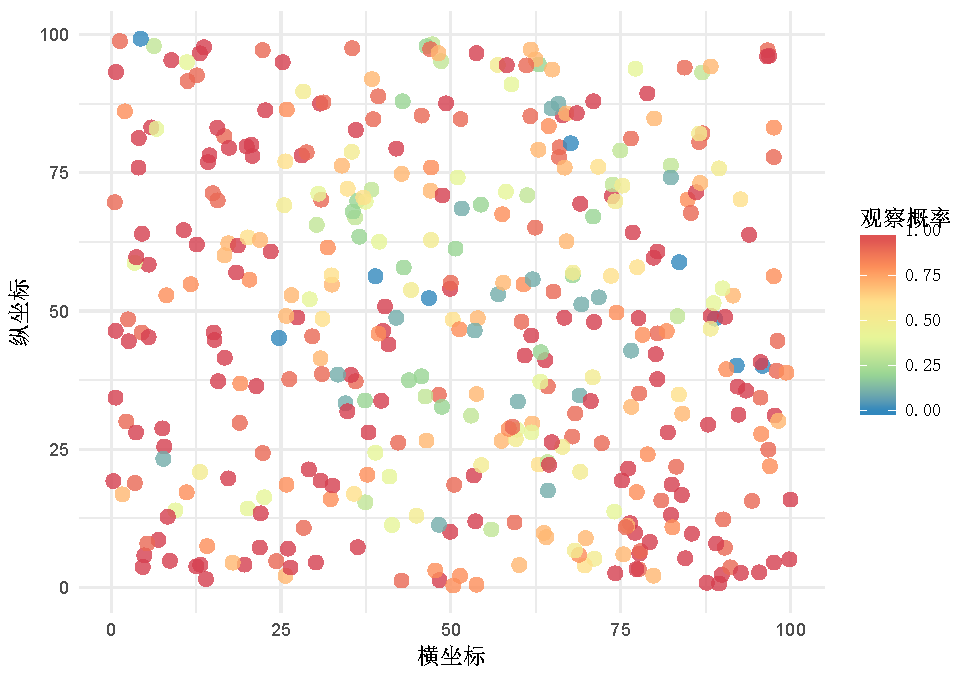
\includegraphics[width=.7\textwidth]{geostatistics_files/figure-latex/simulation-binom-1} 

}

\caption{二项分布}\label{fig:simulation-binom}
\end{figure}

\begin{Shaded}
\begin{Highlighting}[]
\CommentTok{# 响应变量服从泊松分布 }
\NormalTok{## 空间随机效应和协变量同上}
\NormalTok{lambda <-}\StringTok{ }\KeywordTok{exp}\NormalTok{(S}\OperatorTok{$}\NormalTok{data }\OperatorTok{+}\StringTok{ }\NormalTok{data.x }\OperatorTok\StringTok{ }\NormalTok{beta)  }
\NormalTok{pois.data.y <-}\StringTok{ }\KeywordTok{rpois}\NormalTok{(}\KeywordTok{length}\NormalTok{(S}\OperatorTok{$}\NormalTok{data), }\DataTypeTok{lambda =}\NormalTok{ lambda) }

\KeywordTok{ggplot}\NormalTok{(}\DataTypeTok{data =} \KeywordTok{as.data.frame}\NormalTok{(S}\OperatorTok{$}\NormalTok{coords), }
       \KeywordTok{aes}\NormalTok{(}\DataTypeTok{x =}\NormalTok{ x, }\DataTypeTok{y =}\NormalTok{ y, }\DataTypeTok{colour =} \KeywordTok{log}\NormalTok{(pois.data.y }\OperatorTok{+}\StringTok{ }\DecValTok{1}\NormalTok{)) ) }\OperatorTok{+}\StringTok{ }
\StringTok{  }\KeywordTok{geom_point}\NormalTok{(}\DataTypeTok{pch =} \DecValTok{16}\NormalTok{, }\DataTypeTok{size =} \DecValTok{3}\NormalTok{, }\DataTypeTok{alpha =}\NormalTok{ .}\DecValTok{8}\NormalTok{) }\OperatorTok{+}\StringTok{  }
\StringTok{  }\KeywordTok{scale_colour_distiller}\NormalTok{(}\DataTypeTok{palette =} \StringTok{"Spectral"}\NormalTok{) }\OperatorTok{+}
\StringTok{  }\KeywordTok{labs}\NormalTok{(}\DataTypeTok{colour =} \StringTok{"对数}\CharTok{\textbackslash{}n}\StringTok{观察数目"}\NormalTok{,}\DataTypeTok{x =} \StringTok{"横坐标"}\NormalTok{,}\DataTypeTok{y =} \StringTok{"纵坐标"}\NormalTok{)}
\end{Highlighting}
\end{Shaded}

\begin{figure}

{\centering 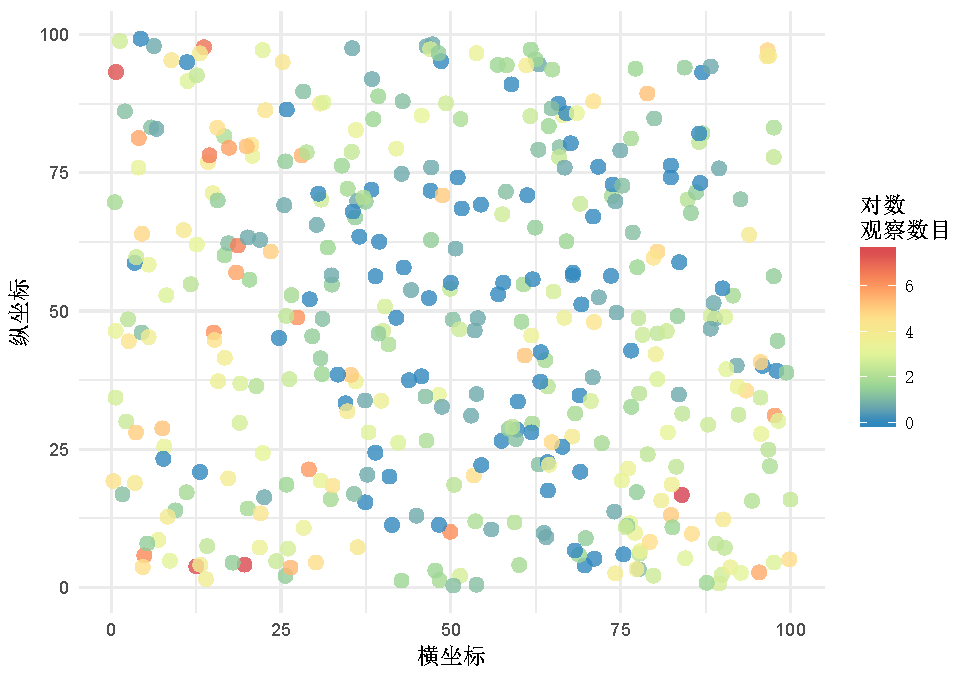
\includegraphics[width=.7\textwidth]{geostatistics_files/figure-latex/simulation-pois-1} 

}

\caption{泊松分布}\label{fig:simulation-pois}
\end{figure}

\[\lambda(x) = \frac{\exp(\mu+S(x))}{1+\exp(\mu+S(x))} \]

\begin{Shaded}
\begin{Highlighting}[]
\CommentTok{# 加载 R 包}
\KeywordTok{suppressPackageStartupMessages}\NormalTok{(\{}
  \KeywordTok{library}\NormalTok{(PrevMap)}
\NormalTok{\})}
\end{Highlighting}
\end{Shaded}

\begin{Shaded}
\begin{Highlighting}[]
\KeywordTok{source}\NormalTok{(}\StringTok{'code/02-Matern-function.R'}\NormalTok{) }
\end{Highlighting}
\end{Shaded}

\begin{center}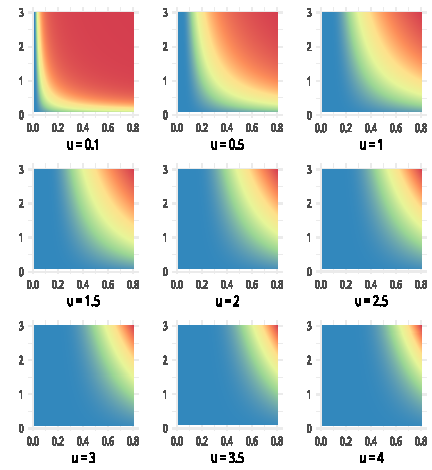
\includegraphics[width=.7\textwidth]{geostatistics_files/figure-latex/matern-1} \end{center}

从蓝到红,值由小变大

\subsection{模拟二项分布数据集}

此处模拟数据集 \texttt{data\_sim} 来自 \texttt{PrevMap}
包,零均值高斯过程 单元格上 \(30 \times 30\) 参数
\(\sigma^2 = 1, \phi = 0.15, \kappa = 2\),块金效应 (nugget effect)
\(\tau^2 = 0\),每个格点上重复实验10次,得到响应变量二项分布的概率值

\begin{figure}[!htb]

{\centering 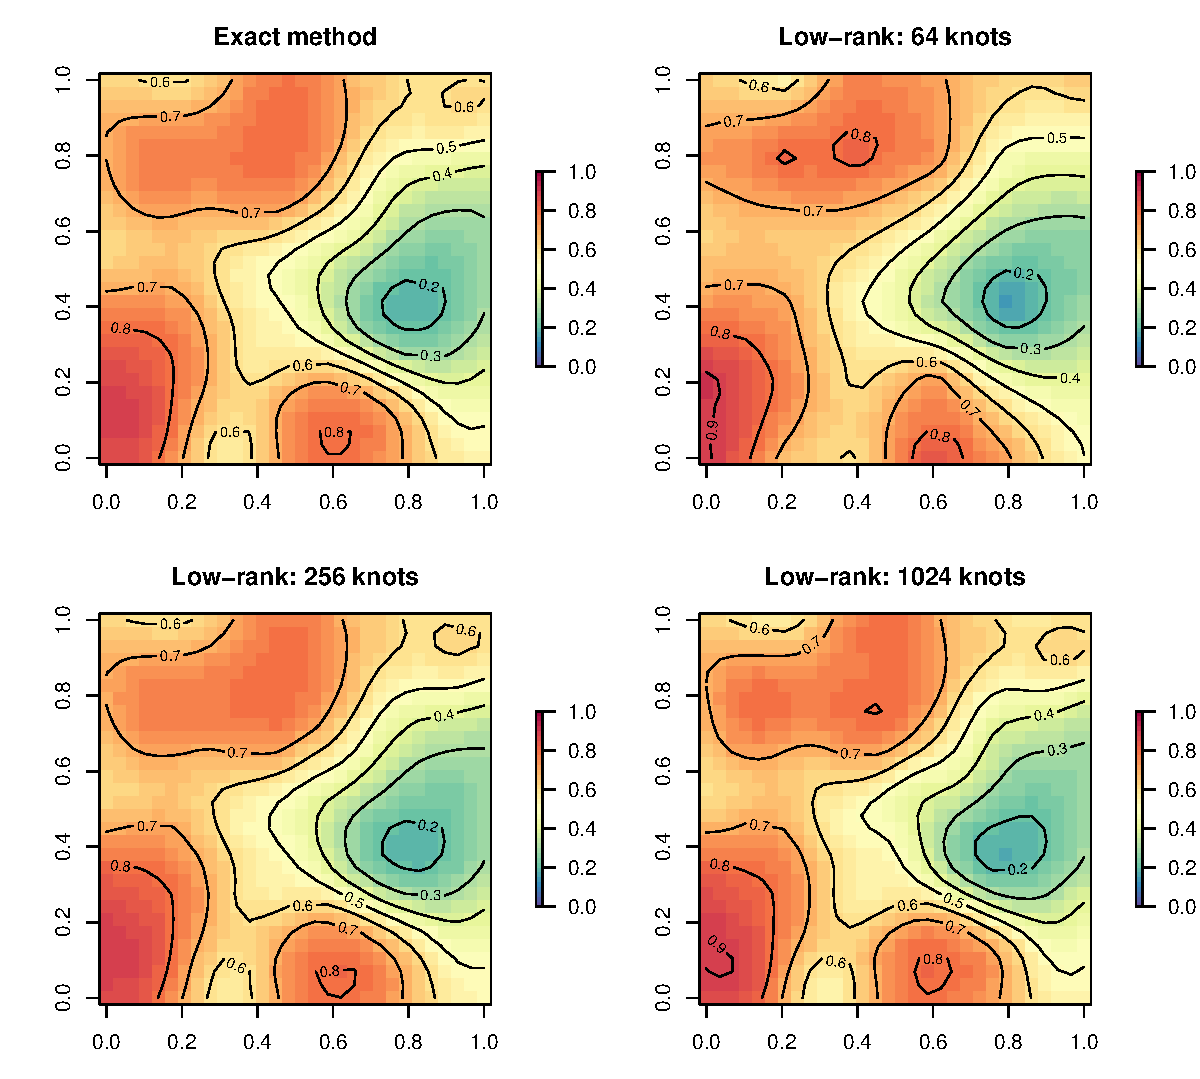
\includegraphics[width=.7\textwidth]{figure/simulation} 

}

\caption{数值模拟}\label{fig:low-rank}
\end{figure}

\renewcommand\refname{参考文献}
\bibliography{refer.bib}


\end{document}
